% !TEX root = ../TechProject.tex

\graphicspath{{Chapter2/}}

\chapter{Machine Learning used in Music Recommendation Systems}

This chapter will answer the following research question:

\textit{What are effective methods for the automated recommendation of songs suitable for adding to a given DJ set?} 

\section{The need for music recommendation systems}
Spotify, SoundCloud, Apple Music and other streaming services give one access to a library of tens of millions songs. Music Recommendation systems are excellent at fitting a user's preference whilst incorporating some level of filtering of an overwhelming amount of songs \citep{bollen_understanding_2010}. 

Music recommendation systems study the habits and tastes of users, and with that information give out suitable recommendations. This aids the listener to discover new songs or artists they otherwise would not have found.

With this potential, a well made recommendation system could be a make or break for choosing one streaming service from another. For this reason a lot of research gets put into recommendation systems as an attempt to retain engagement. 

 With recommending music, a lot of sub conscious factors come into play on what a user wants to listen to at a given time. This can range from characteristics and mood of the listener, to what they get up to in day-to-day life \citep{ferwerda_personality_2015, rentfrow_re_2003, gillhofer_iron_2015, wang_context-aware_2012}.  The users environment can have an affect as well \citep{kaminskas_location-aware_2013}. Observing a user made playlists also can reveal a lot on what groups of songs work for particular situations \citep{zheleva_statistical_2010, mcfee_hypergraph_2012}.
 
 A necessity for making a recommendation system suited for a type of product is taking into consideration the common place attributes of the product. Music lends itself to having a specific method due to short duration and high emotional connection. A recommendation system that uses these attributes to its advantage will be more successful than ones that don't.

\section{Collaborative filtering}

Collaborative filtering guesses a user's taste by looking at similar user-item connections. Using an explicit example, if a user rates something highly, it can provide similar suggestions from looking at the ratings of other users\citep{celma_recommendation_2010}.

\begin{figure}[H]
	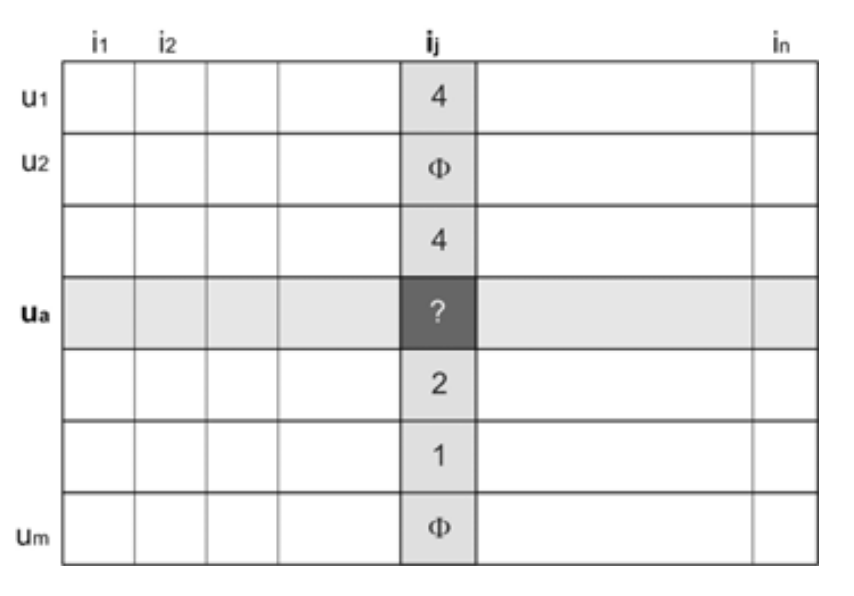
\includegraphics[scale=0.65]{images/collaborative_filtering}
	\centering
	\caption{User-item matrix used for collaborative filtering \citep{celma_recommendation_2010}} 
	\label{fig:figure}
\end{figure}

Collaborative filtering works by taking a matrix of users and items where some form of interaction is measured. Examples of interaction's could be plays of a song, rating of a movie/product or screen time on an app. In figure 2.1, i represents items, and u is users.

The first known use of collaborative filtering is with Goldberg's "Tapestry" system, a mailing list filter where users collectively decide which type of emails get the most importance \citep{goldberg_using_1992}. The first instance of collaborative filtering being used for music recommendations was in a system called Ringo where users would rate music (album, songs, artists, etc.) and get recommendations pulled from similar users \citep{shardanand_social_1995}. 

Despite the prevalence of deep learning and neural networks, collaborative filtering is still used in today's state of the art recommendation systems. The winner of the 2018  RecSys Playlist Continuer Challenge used a combination of collaborative filtering and deep learning in their model \citep{volkovs_two-stage_2018}.

Collaborative filtering can be divided into the following types:

\begin{enumerate}
	\item Explicit Feedback
	\item Implicit Feedback
	\item Item Based
	\item User Based
\end{enumerate}




\subsection{Explicit Feedback}

 Explicit feedback is when a user is asked for some form of measurement about the likeability of a product \citep{celma_recommendation_2010}. The RACOFI (Rule-Applying Collaborative Filtering) system uses explicit feedback. Collaborative filtering with ratings finds initial recommendations. Then the system applies logic rules to decipher further the most suitable recommendations \citep{anderson_racofi_2003}.  Its added logic rules implicitly change the user’s previous ratings. Other recommendation systems started having similar rules, including Indiscover and Slope One \citep{celma_music_2010, lemire_slope_2007}. Ringo and many of the first music recommendation systems that use collaborative filtering use explicit feedback for their data. 

\subsection{Implicit Feedback}

Recommendation systems that take only implicit feedback will focus on what the listener interacts with, rather than asking them for their opinion of the content. The main reason implicit feedback is frowned upon is that using this method doesn't give a scale of enjoyability of the content, in the context of music, just whether the user listened to said song or artist how many times \citep{celma_recommendation_2010}. Spotify is an example of this, if another person uses their account or if they left a device on autoplay as well on mute. However, collecting implicit data is a lot easier because it just requires engagement with the said application to get valuable information. 

There is also a lot to be found with implicit data. In 2018, a music recommendation system produced an effective recommendations derived from the time of day in which users listened to music \citep{sanchez-moreno_incorporating_2018}. Takama et al took this a step further by using time of day as well as, nationality and content features found through Spotify \citep{takama_context-aware_2021} 

\subsection{Item-Based Neighbourhood }

Item-based neighbourhood is when similarities for a given item are found based on the user's previous item ratings. First one calculates the similarity among the item's ratings and then the prediction of a given items rating is calculated. Figure 2.2 shows a matrix with ratings from  $u_{2}, u_{i}$ and $u_{m-1}$. For finding similarities between $i_{i}$ and $i_{k}$, we only take $u_{2}$ and  $u_{i}$ into consideration when using item based neighbourhood because they have rated both item $i_{i}$ and $i_{k}$.  

\begin{figure}[H]
	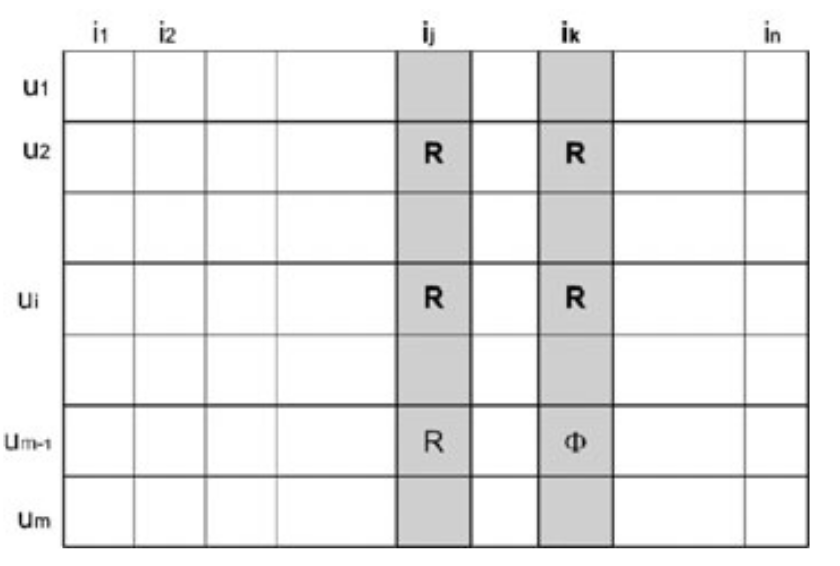
\includegraphics[scale=0.65]{images/neigbourhood_based}
	\centering
	\caption{Matrix showing given ratings. \citep{celma_recommendation_2010}} 
\end{figure}

There are many ways to calculate how similar two items, examples being cosine similarity, Pearson correlation or adjusted cosine similarity. Equation 2.1 shows cosine similarity, the inner product space is taken into account by calculating its similarity.

\begin{equation}
		sim(i , j) = cos( \textbf{i}, \textbf{j} ) = \frac{ \textbf{ i }, \textbf{ j }}{ || i || * || j || } = \frac{ \sum_{ u \in U } r_{ u, i }, r_{ u, j }} { \sqrt{ \sum _{  u \in U } r^{2}_{ u , i}} \sqrt{ \sum _{  u \in U } r^{2}_{ u , j}}}
\end{equation}

Cosine similarity is not advised for comparing how similar recommendations are because users often have their own personal ranges when it comes to rating. Adjusted cosine similarity is good because it subtracts the users average from each co-rated pair, this handles users personal ranges appropriately \citep{sarwar_item-based_2001}. Equation 2.2 for adjusted cosine similarity is shown.

\begin{equation}
	sim(i , j) = \frac{ \sum_{ u \in U } ( r _{ u, i } - \bar{r} _{u} ) ( r _{ u, j} - \bar{r} _{u} ) } { \sqrt{\sum_{ u \in U } ( r _{ u, i } - \bar{r} _{u} )^2} \sqrt{\sum_{ u \in U } ( r _{ u, j } - \bar{r} _{u} )^2}}
\end{equation}

Once similarities of the users previous ratings are calculated, the next step is to predict how the user would rate the item in question. A way of doing this is to calculate a weighted sum of the user's previous item ratings. Calculating the weighted sum predicts how the user would rate the given item based on the ratings of similar items. Weighted sum is scaled to ensure the predicted rating is in an appropriate range\citep{sarwar_item-based_2001}. Allowing $ S^{k}(i;u)$ to equal the list of items i user u has rated, equation 2.3 shows how the predicted value is found.

\begin{equation}
	\hat{r} _{u,i} = \frac{ \sum _{ j \in S^{k}(i;u)} sim(i , j) r _{u, j}}{\sum _{j \in S^{k}(i;u)} sim(i , j)}
\end{equation}
\\
\\
\\
Another way of predicting a rating is using Regression. Predictions are made with the same equation as weighted sums, but approximate values based on a linear regression model are used instead of "raw" rating values. Allowing target items be \textit{i} and similar item N by $R_{i}$ and $R_{N}$, 2.4 shows the linear regression model \citep{sarwar_item-based_2001}.

\begin{equation}
	\bar{R'} _{N} = \alpha \bar{R}_{i} + \beta + \varepsilon
\end{equation}

Parameters of the regression model ($\alpha , \beta$) are found by going through the rating vector pairs, and $\varepsilon$ is the error of the model \citep{sarwar_item-based_2001}.

\subsection{User Based}

User-based neighbourhood is when you look for users who rate similarly to see whether item i is similar to user u. This differs from Item Based because user based skips calculating similarity of co-rated items \citep{pinela_recommender_2017}. Equation 2.5 shown is similar to 2.3 but instead it sums a list of similar users.

\begin{equation}
	\hat{r} _{u,i} = \bar{r}_{u} + \frac{ \sum _{v \in S(u)^{k}} sim(u ,v) ( r_{v, i} - \bar{r}_{v})}{\sum _{v \in S(u)^{k}} sim(u , v)}
\end{equation}

As mentioned previously, pearson correlation, cosine similarity can be used to calculate similarity ($sim(u ,v)$). Another way of calculating similarity is matrix factorisation

\subsection{Matrix Factorisation}

\begin{figure}[H]
	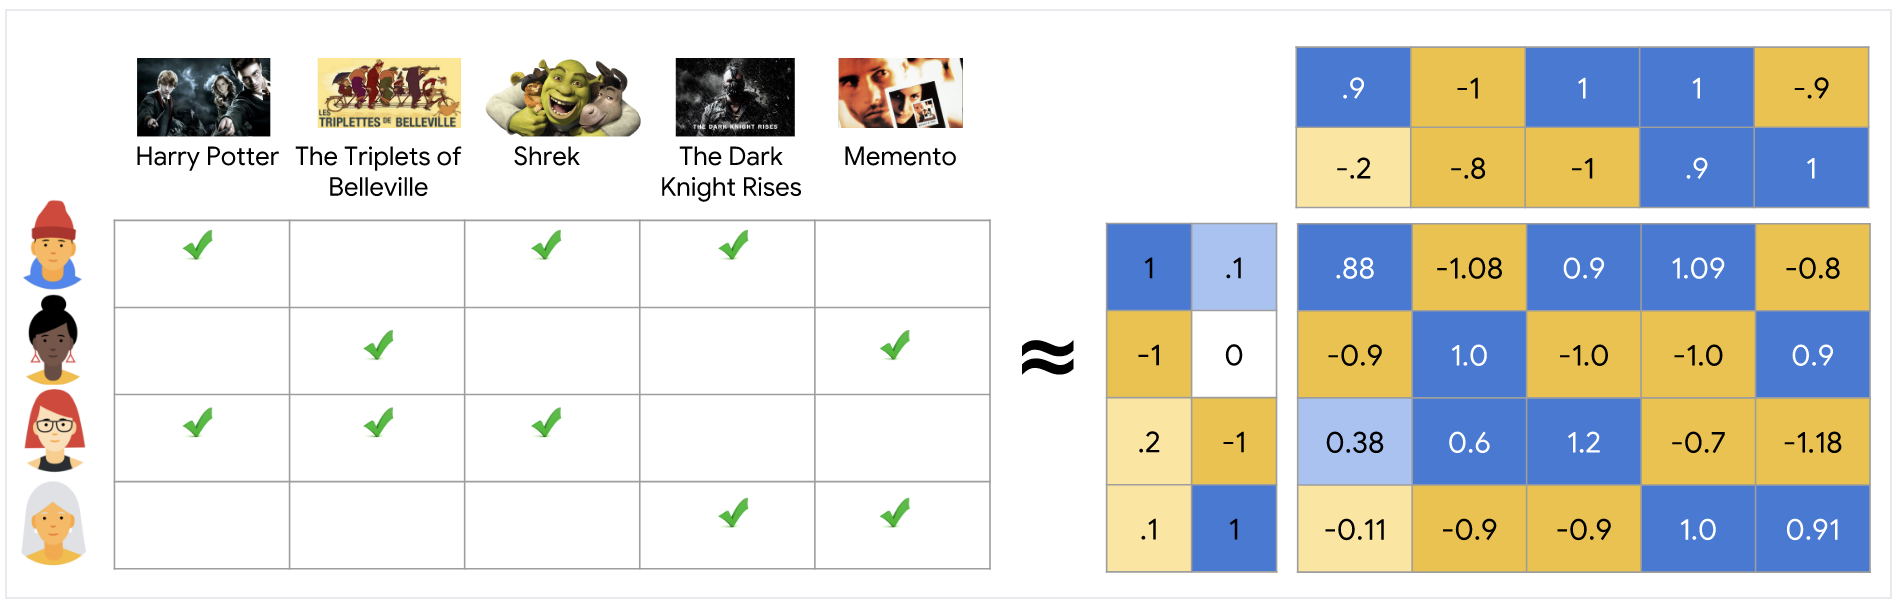
\includegraphics[scale=0.45]{images/matrix_factorisation_example}
	\centering
	\caption{A Movie Rating example of matrix factorisation  \citep{httpsdevelopersgooglecom_matrix_2023}} 
	\label{fig:figure}
\end{figure}

When one has a matrix of plays for each user and song, matrix factorisation can be used to find recommended songs. Matrix factorisation processes the matrix into 2 vectors. These vectors are from factors of the user item rating patterns \citep{koren_matrix_2009}. Figure 2.3 and 2.4 illustrates how, where latent factors (products used to factorise matrix) are used to approximate and predict users ratings of movies. 

\begin{figure}[H]
	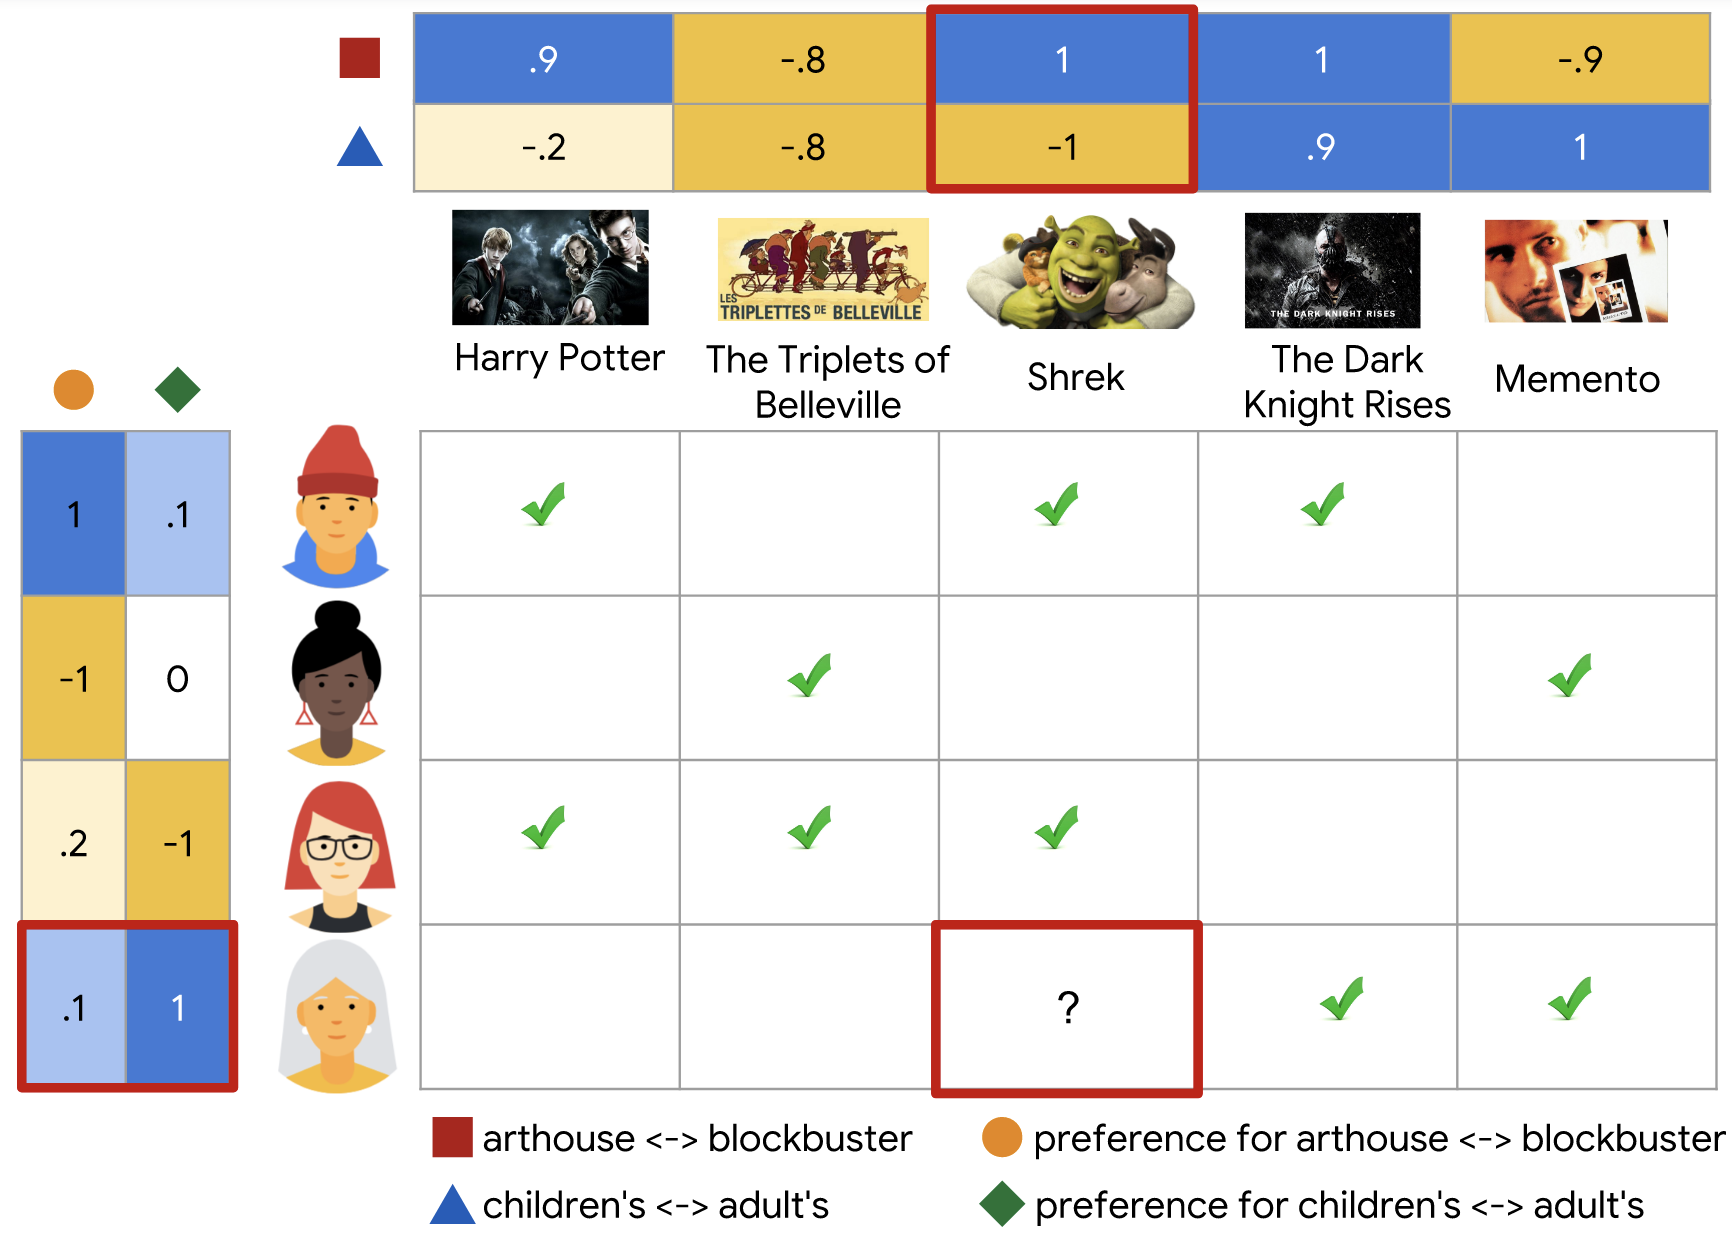
\includegraphics[scale=0.45]{images/latent_factors}
	\centering
	\caption{What latent factor values can tell us about user/item interactions \citep{httpsdevelopersgooglecom_matrix_2023}} 
	\label{fig:figure}
\end{figure}

This is useful for a sparse matrix (when most user/item interactions are zero), because it shows information that the matrix alone does not.  One can see trends of preference within the latent factors. Because it reduces the dimensionality of a given matrix. Matrix factorisation also requires less processing power than methods that search through the raw matrix. 

There are different ways of factorising a matrix. An example of one is Singular Value Decomposition (SVD). Equation 2.6 shows this with $U$ and $V$ matrices for a given number of dimensions,  where M is the approximated matrix:

\begin{equation}
	M = U \sum V ^{T}
\end{equation}

Alternating Least Squares, is a computational safe way to calculate M. It works by alternating between estimating the U and V matrices until it reaches closely to the value of M. Stochastic gradient (another method for calculating M) repetitively uses random bits of data to approximate U and V \citep{koren_matrix_2009}. 

When the matrix is split up, the predicted rating can be calculated from the user and item feature vectors. 


Looking at the latent factors one can find  similar items using a cosine similarity. When working with sparse data, its favourable to use Alternating Least Squares because of its greater potential for parallelisation (working out calculations simultaneously) \citep{koren_matrix_2009}.

\subsection{Limitations}
Despite its popularity, Collaborative filtering has limitations as a recommendation method.

\textbf{Sparse Data - }Not every user has listened to every song. This means in data sets, having a sparsity of around 98-99 \% is very common \citep{celma_recommendation_2010}.

\textbf{Grey sheep - }This is when a user has a unique taste that is dissimilar to most other users, making it hard to stem recommendation's from. This is a common problem with datasets that are very sparse \citep{claypool_combining_1999}.

\textbf{Cold Start and Early Raters - } The term cold start refers to new items whilst early raters refers to new user \citep{avery_recommender_1997}. When there are new users or items, there is little data associated with them so it is challenging to come up with suitable recommendations based on either the user or item. 

\textbf{Popularity Bias - } Collaborative filtering does not take into account information about the item, only user interactions with it. This means that it has a bias towards popular items \citep{celma_recommendation_2010}.

\textbf{Feedback loops - } When users interact with items that are recommended through Collaborative Filtering, based on previous user item interactions, it strengthens the initial recommendations more and creates a loop \citep{sanchez-moreno_incorporating_2018}.

\section{Content Based Filtering}

Content Based Filtering works by looking at the characteristics of a given item and see if it matches the preference of the user. Recommendations stem from the given information about the item, not what other users interact with. Item's information is found and then is used to find similar items\citep{casey_content-based_2008}. Music recommendation systems stem from song information that aligns with the users taste \citep{aucouturier_music_2002, logan_music_2004}. 

Early uses of content based filtering were text based, because of its ease of information extraction, An example of this is the PRES system \citep{van_meteren_using_2000}. Machine learning has enabled extraction of information from complex formats like images or audio. Models like "Xception" have proven successful at extracting audio features from songs \citep{chollet_xception_2017, singh_robustness_2022}.

There has been a lot of research on extracting musical components from an audio file \citep{ribecky_multi-input_2021, zhao_musical_2022}. Recent developments have shown successful extractions of genre and structure with the MusicBERT Model \citep{zhu_musicbert_2021}. It's found that MIDI extraction from songs can aid to give better solutions for less popular songs, helping eliminate the cold start problem \citep{yadav_improved_2022}.

Content based filtering looks at how similar the attributes of each item is when finding recommendations. It's decision making doesn't use subjective factors, like user behaviour. An item is used as a vector made of its defined values of attributes, where the distance between other items can be found. Distance can be calculated using Euclidean, Manhattan, Chebyshev, cosine distance and Mahalanobis distance. With two feature vectors equalling $x$ and $y$, equations are found below.
\\
\\
\textbf{Euclidean Distance:} The distance between two points.
\begin{equation}
	d(x,y) = \sqrt{\sum _{i=1} ^{n}(x_{i} - y_{i})^{2}}
\end{equation}

\textbf{Manhattan Distance:} The sum of the absolute differences between two vectors.
\begin{equation}
	d(x,y) = \sum _{i=1} ^{n} | x_{i} - y_{i} |
\end{equation}

\textbf{Chebychev Distance:} The greatest difference between two vectors.
\begin{equation}
	d(x,y) = man_{i} = _{1 . . n} | x_{i} - y_{i} |
\end{equation}

\textbf{Mahalanobis Distance:} The distance between a point and a distribution of points.
\begin{equation}
	d(x,y) = \sqrt{ ( x - y )^{ T } S^{ -1 } ( x - y ) }
\end{equation}

Euclidean, Manhattan and Chebychev distance are used when there is little relationship or correlation between attributes. If there is correlation, its advised to use Mahalanobis distance \citep{celma_recommendation_2010}.

Equation 2.11 is a delta function ($\delta $) and is used when attributes aren't measured numerically. When two attributes match it equals zero, other wise it equals 1.

\begin{equation}
	d(x,y) = \omega \sum _{ i = 1 } ^{ n } \delta (x _{i}, y _{i})
\end{equation}

Content based filtering overcomes the problems collaborative filtering has of being able to rate items that previously haven't had any ratings. Its also able to adapt to any changes in the users preference quickly \citep{isinkaye_recommendation_2015}. For users who don't want to share their data they can get suitable recommendations as well \citep{k_you_2006}.

\subsection{Limitations}
The cold start and grey sheep problem also occur in content based filtering. Popular items usually have better defined features, and older users have better represented features.

\textbf{Novelty Problem - } This is when the user is recommended items too similar to the one they already have, an application would need some way of diversifying recommendations to overcome this \citep{celma_recommendation_2010}.

\textbf{Retrieving metadata - } Despite recent improvements in extracting musical information \citep{vall_feature-combination_2019, singh_novel_2022}. This data is used in mainly in deep neural networks or hybrid models. Obtaining rich enough meta data to rely on Content Based Filtering alone is still not reliable.

\textbf{Suggestions not opinionated- } It doesn't take into the account the opinions of users, only description of what the item is. This may lead to some poor quality recommendations that only relying on observing features would obtain \citep{celma_recommendation_2010}.  

\section{Clustering}

Another method of finding similar items is Clustering. Clustering is when one  groups a collection of data objects, so that some objects clustered together are very similar, while other clustered objects are not alike. Similarity is then evaluated based on chosen parameters \citep{ferretti_clustering_2018}. A popular algorithm is the k-mean cluster where each cluster is representerd by a mean value of the object \citep{han_data_2006}. A model that uses an altered version of k clustering limits the randomness in the suggestion this method generates \citep{chang_personalized_2017}.


\section{Diversity issue}

Recommendation systems are used extensively by the majority of Spotify users \citep{spotify_spotify_2020}. However, there are a subsection of users who, despite huge breakthroughs, don't rely on algorithmic means of discovering music. In 2020, a study done found that users with more diverse tastes would find music in non algorithmic ways \citep{anderson_algorithmic_2020}. Users with less diverse taste relied on algorithms for recommendations. Users who's taste became more diverse, occurred from non algorithmic ways of finding music.

A reason for this is the small amount of listeners who have a diverse taste, lots of music recommendation systems don't focus on a specific type of person when training a model \citep{laplante_improving_2014}.

It's argued that the way classification is handled in music could also be a reason \citep{porcaro_diversity_2021}. The classification of music is a debate that has been passed from generations \citep{moles_sociodynamique_2019, dimaggio_classification_1987, bourdieu_distinction_2010}. In the context of a recommendation system, a genre being treated as a "tag" usually pushes its social and cultural relevance to the side \citep{porcaro_diversity_2021}. The act of a machine understanding a concept as subjective as genre is one that has proven challenging \citep{nurnberger_survey_2014}. Vlegels attempts to overcome this by organise groupings based on user artist relationship, rather than an artists genre \citep{vlegels_music_2017}.

This problem existing could be a reason for the continued need for "curation", the act of having a professional spot interesting things and document them to consumers \citep{barna_perfect_2017}. With this comes the role of a DJ, whom before recommendation systems existed, were doing just that \citep{percival_music_2011}. 

Recently there has been attempts of integrating DJs in streaming services.  An example of DJ's and algorithmic centric streaming apps coexisting is Apple Music's Beats 1 Radio station. The subscription service allows access to a radio station of the most popular artist and DJs in the western world broadcasting shows, providing entertaining commentary and selected musical recommendations \citep{dms_apple_2020}. Another is Spotify's curated playlists, and more specifically there track ID's series, where they get established DJs to make a huge ever changing playlist of songs they play out live \citep{spotify_introducing_2020}.  Seeing this type of content shows how a company can pedal a term like "curation" in the music world and see it as a necessity \citep{barna_perfect_2017}. One can see this in the rise of internet radio as well.  

Internet radio is a strangely thriving industry which is expected to have an net worth of \$9.2 Billion by 2030 \citep{market_research_future_internet_2022}. This boom has seen growth within DJ centric radio stations \citep{gillett_how_2021}. Its popularity can be drawn from increased speeds in mobile data, and choice of stations, but one can see that curation is a big draw to its appeal \citep{nts_2023}.

Despite the vast amount of data surrounding DJ sets, there's been little research on using DJ sets to train algorithmic models. A unique instance of this is found in Chows recommendation system made out of the many DJ mixes found on MixesDB. The application inputs a single song and outputs similar songs found through the dataset \citep{chow_music_2020}. Finding recommendations from multiple songs or another DJ set is something that has been previously unexplored, and could provide with solutions with assuring a exciting level of diversity that is missed in many recommendation systems.


\section{Summary}
The theory behinds recommendation systems were introduced and explained, with examples of current day models that use them. With its success, it was addressed from a survey that recommendation systems aren't commonly used with users with "diverse" music taste. The continued use of internet radio, DJ sets and curated playlists affirmed the findings of this survey. It was concluded that little research has been done on training an algorithmic model from DJ sets, potentially providing a recommendation system that would appeal to listeners with diverse taste. 

% note that \Blindocument has 5 numbered levels, despite setting secnumdepth above. I (and many style guides) would suggest using no more than 3 numbered levels (incl. the chapter), with the option of a fourth unnumbered level.